\documentclass[a4paper]{report}
%Use this line instead if you want to use running heads (i.e. headers on each page):
%\documentclass[runningheads]{llncs}
\usepackage[german]{babel}
\usepackage[utf8]{inputenc}
%\usepackage{multimedia}
\usepackage{mathtools}
\usepackage{paratype}
\usepackage{float}
\usepackage{graphicx}
\usepackage{caption}
%\usepackage{natbib}
\usepackage{subcaption}
\usepackage{nameref}
\usepackage{url}
\usepackage{hyperref}
\usepackage{xcolor}
%\usepackage[style=mla]{biblatex}

\usepackage[affil-it]{authblk}

\captionsetup{compatibility=false}
\DeclarePairedDelimiter{\abs}{\lvert}{\rvert}


\usepackage{ifthen}

%remove [] around bibitems
\makeatletter
\renewcommand\@cite[2]{%
	Ref.~#1\ifthenelse{\boolean{@tempswa}}
	{,#2}{}
	%{, \nolinebreak[3] #2}{}
}
\renewcommand\@biblabel[1]{#1}
\makeatother

\begin{document}
	
	\title{DRONARCH - Drone Supported Reconstruction Of Natural Environment and Archaeological and Cultural Heritage}
	
	\author{Niclas Scheuing}
	\date{2014}
	\affil{Institut für Archäologische Wissenschaften, Archäologie der Römischen Provinzen, Universität Bern}
	
	\pagenumbering{roman} \setcounter{page}{1}
	\maketitle
	\tableofcontents
	\clearpage
	\pagenumbering{arabic} \setcounter{page}{1}
	
	\chapter{Einleitung}
	Ziel der Archäologie ist das Bewahren und Verstehen von materiellen Spuren vergangener Zeit. Dazu gehören Ausgrabungen, die gezielt archäologische Befunde freilegen und diese dabei teilweise zerstören. Die Information, die Befunde liefern, können also nicht im Original erhalten werden, sondern müssen laufend dokumentiert werden. Diese Dokumentation bildet die Grundlage für die Interpretation und Auswertung durch heutige und zukünftige Archäologen.
	Das Erfassen dieser Informationen ist dadurch ein ausgesprochen wichtiger Punkt und die kritische Diskussion seiner Methodik verdient einige Aufmerksamkeit.
	
	\section{Definition}
		Dokumentation ist in erster Linie Erfassen von möglichst vielen und möglichst exakten Informationen. Generalisierung und Selektion ist nur notwendig, wenn die vorhandenen Informationen Mangels Technik, Zeit, Geld oder Lagermöglichkeiten nicht festgehalten werden können und ein Abwägen des Nutzen-Kosten Verhältnisses nötig ist. Ist es etwa sinnvoll Tonnen von Dachziegeln zu reinigen, fotografieren, zeichnen und archivieren, oder reichen einige repräsentative Exemplare?
		Idealerweise sollten aber \emph{alle} Informationen erhalten bleiben.
		
	\section{Klassische Dokumentation}
		Der Archäologische Dienst des Kantons Bern (ADB) schriebt in seinem Handbuch: ''Zeichnungsdokumentation, Beschrieb und Fotodokumentation sind die drei Standbeine der Grabungsdokumentation.'' \citeu{adb:handbuch}.
		
		\subsection{Fotodokumentation}
			Fotos bilden visuelle Informationen mit wenig Verfälschung ab. Sie zeigen die Situation auf eine sehr natürliche Weise und sind wenig von Interpretation beeinflusst.
			Beim Fotografieren können die Wahl von Standort, Bildausschnitt, Objektiv und Lichtverhältnis einen gewissen Einfluss auf deren Interpretation haben. Zudem ist die erreichbare Qualität eines Fotos durch die verwendete Ausrüstung beschränkt.
			So können wichtige Details verloren gehen, wenn schlecht Fotografiert werden, oder die Fotos sind schwierig in Kontext zu setzen, wenn es an Übersichtsaufnahmen und Aufnahmedatum fehlt.
			Seit digitale Kameras die analoge Fotografie abgelöst haben, ist die Menge an Foto und deren Verfügbarkeit stark gewachsen\footnote{Der online Bilderdienst Flicker kann als Referenz betrachtet werden: \cite{flickr:number}}. Das ist im Sinne einer zeitlich und räumlich lückenlosen Dokumentation.
			Doch es führt möglicherweise auch zu einer grossen Menge an wenig informativen Fotos, die insgesamt zwar schneller und einfacher gemacht worden sind, aber letztlich weniger aussagekräftig sind als weniger dafür bessere Fotos.
			Gute Fotos zu machen, daraus eine Auswahl zu treffen und diese mit der restlichen Dokumentation in Kontext zu setzten, kann ein beachtlicher Aufwand sein.
			Automatisierte Unterstützung beim Erfassen und Auswerten könnte diesen Prozess deutlich effizienter machen.

		\subsection{Zeichnungsdokumentation}
			Zu Zeichnungen schreibt der ADB in seinem Handbuch \citeu{adb:handbuch}: ''Man kann nur zeichnen was man versteht.''
			Zeichnerische Dokumentation generalisiert, hebt Wichtiges hervor und lässt Unwichtiges weg. Für die Unterscheidung zwischen Wichtig und Unwichtig ist eine Interpretation erforderlich.
			Dies führt dazu, dass das Erstellen der Dokumentation vor Ort viel Zeit erfordert. Somit enthält eine Zeichnung nicht nur die Abbildung eines Befundes, sondern auch eine Interpretation dazu. Dieser reichere Informationsgehalt ist zwar für die spätere Interpretation sehr nützlich, stellt aber auch eine Verfälschung der realen Befundsituation dar.
			
		\subsection{Beschrieb}
			Fotos und Zeichnungen enthalten in erster Linie visuelle Informationen. Weitere wichtige qualitative Merkmale, etwa Materialien und Beschaffenheit, werden in Text festgehalten.
		
			
	\section{Fehlende Dimension}
		Fotos und Skizzen sind zweidimensionale (2D) Beschreibungen einer dreidimensionalen (3D) Realität. Es ist eine Projektion nötig, die um eine Dimension reduziert. Fotografie verwendet naturgemäss eine perspektivische Projektion (Zentralprojektion), für Skizzen hingegen verwendet man oft auch eine orthographische Projektion (Parallelprojektion).
		In jedem Fall geht eine ganze Dimension an Informationen verloren und muss mittels Abbildungen verschiedener Perspektiven vom Betrachter rekonstruiert werden.
		Dies erschwert die Interpretation dieser Form von Dokumentation und bedingt eine gute Wahl der Perspektive beim Erstellen der Abbildungen.
		
		Soweit wird die 3D Realität mittels verschiedener Projektionen und Techniken auf zwei Dimensionen abgebildet und im Kopf des Archäologen wieder in 3D rekonstruiert.
		Deutlich einfacher und intuitiver für den Betrachter ist es die 3D Struktur direkt abzubilden, zu speichern und zu betrachten.
	\chapter{Motivation}
	Die Idee 3D Strukturen in drei Dimensionen zu Erfassen und Darzustellen ist naheliegend, bedingt aber Aufnahmegeräte und eine Datenrepräsentation, die 3D Inhalte unterstützen. Dazu kommen neben aufwändigen Miniaturen nur computergestützte Verfahren in Frage.
	
	\section{Ziel dieser Arbeit} \label{frag:ziel}
		In dieser Arbeit werden Verfahren zur 3D Dokumentation präsentiert und deren technischen \emph{Möglichkeiten} und \emph{Nützlichkeit} für die Archäologie diskutiert.
		Insbesondere wird \emph{Structure from Motion} (SfM, siehe \autoref{sfm}) als einfaches und günstiges Verfahren zum Erstellen von 3D Modellen betrachtet und mit anderen Methoden verglichen.
		Anhand einiger Fallstudien soll die Möglichkeit der Integration in bestehende Grabungs- und Dokumentationspraxis und deren Vor- und Nachteile überprüft werden.
		Die Hauptpunkte sind dabei:
		\begin{itemize}
			\item
			\emph{Mehrwert} der 3D Dokumentation gegenüber der 2D Dokumentation
			\item
			\emph{Aufwand} zum Erstellen eines 3D Modells
			\item
			\emph{Qualität} und Fehler eines gewonnen Modells
			\item
			\emph{Integration} anderer Dokumentationen, insbesondere GIS-Daten
		\end{itemize}
	
	\section{Kriterien} \label{frag:kriterien} %TODO: Referenzen aktualisieren
		Einer Diskussion aufgrund praktischer Resultat muss eine theoretische Reflexion der Möglichkeiten und Präzisierung der Fragestellung und  der Kriterien zur Auswertung vorangehen.
		Die Motivation für die Nutzung von SfM in der Archäologie ist eine Verbesserung der Dokumentation. Es muss allem voran erst
		\subsection{Mehrwert}
			Der Mehrwert einer 3D Rekonstruktion hängt in erster Linie von dessen Qualität ab, je exakter das Modell, desto mehr Informationen sind darin dokumentiert.
			
			Wenig detaillierte Modell visualisieren geometrischen Zusammenhänge, Dimension, Orientierung und grob die farblichen Unterschiebe innerhalb einer Grabung. Siehe [TODO:Bild]. Die räumliche Darstellung vereinfacht es sich einen Überblick zu verschaffen und weitere Fragmente der Dokumentation zueinander in Bezug zu setzten.
			Zudem lassen sich 3D Modell gut für Öffentlichkeitsarbeit verwenden, da sie auch dem ungeübten Betrachter einfach und intuitiv die Situation aufzeigen.
			
			Bei höherer Qualität der Rekonstruktion sind auch Details wie Mauerfugen und kleinere Artefakte zu sehen. Siehe [TODO:Bild]. Als Dokumentation, im Sinne vom Erfassen möglichst vieler und genauer Informationen, ist dies ein sehr kompaktes und praktisches Format, da es neben den visuellen Informationen einer Fotografie auch die metrischen Informationen eines Planes und die geometrische Struktur mehrerer Skizzen vereint. 
			
		\subsection{Aufwand}
			Der zeitliche Aufwand besteht zum Einen in einem aktiven Aufwand, das Aufnehmen der Fotos, das Starten der Software und eventuelle Nachbearbeitungen. Zum Andern besteht der passive Aufwand aus Rechenzeit, die ohne Nutzereingabe benötigt wird zum berechnen des Modells.
			
			Der materielle Aufwand beschränkt sich auf eine Kamera und einen Computer. An den Computer sind keine besonderen Voraussetzungen gestellt, aber die Berechnung kann durch bessere Hardware stark Beschleunigt werden.

		\subsection{Qualität}
			Dabei ist in erster Linie der Fehler oder die Korrektheit des Modells interessant. Die Korrektheit lässt sich nicht schlüssig beweisen, da dazu ein korrektes Referenzmodell existieren müsste.
			Stattdessen gibt es verschiedene Methoden den Fehler zu schätzen.
			
			\subsubsection{Referenzpunkte}
				Bevor die Fotos gemacht werden, misst man Referenzpunkte ein und markiert diese. Im fertigen Modell sind diese Punkte erkennbar und dienen einerseits zum Skalieren, Orientieren und Positionieren des Modells und andererseits zum Berechnen des Fehlers. Die Abweichung kann dann für jeden Punkt und für das gesamte Modell berechnet werden.
				
				Verhoeven \etal \citeu{ARCM:ARCM667} verwenden dazu auf den Fels aufgemalte Markierungen, die auf den Luftaufnahmen zu erkennen sind und berechnen daraus den RMSE (Root Mean Square Error).

			\subsubsection{Vergleich mit anderen Methoden}
				Zusätzlich zum durch SfM erstellten Modell, wird mittels einer anderen Methode ein zweites Modell erstellt, das als Referent dient. Dabei ist a priori nicht klar welches Modell der Realität besser entspricht, es ist also kein wirklicher Vergleich mit der Realität.
				
				Galeazzi \etal \citeu{arch:laser_vs_dense_stereo} verglichen Laser Scans und MvS. Laser Scans sind etabliert und bekannt für eine hohe Genauigkeit und eignet sich deshalb sehr gut als Referenz.
			
		\subsection{Integration}
			Die Verbindung des 3D Modells und der bestehenden Dokumentation ist hauptsächlich eine Frage des Aufwandes während der manuellen Nachbearbeitung. Mit entsprechender Software kann das Modell mit Koordinaten aus GIS versehen oder 2D Ansichten aus dem Modell extrahiert werden.
			
			Dellepiane \etal schreiben dazu: ''This method [SfM und MvS], if properly combined with other technologies such as Total Station or GPS (GNSS), can generate very powerful spatio-temporal information.'' \citeu{arch:dens_ster_excav}
		
	\section{DRONARCH}
		Als technische Grundlage für die Fallstudien dient die Software \dronarch\ \citeu{dronarch:github}, die im Rahmen dieser Arbeit geschrieben wurde und das SfM Verfahren verwendet.
		Im Gegensatz zu bestehenden Publikationen, die sich mit SfM in der Archäologie beschäftigen \citeu{arch:laser_vs_dense_stereo, ARCM:ARCM667, ARP:ARP399, TUW-210216, DeReu20131108, the_cave, altai}, verwendet und publiziert \dronarch\ nur Open Source Software und will ein Werkzeug bieten mit wenig Geld und Zeitaufwand 3D Modell für den archäologischen Einsatz zu erstellen.

	
	\chapter{Bestehende Arbeiten}

	\chapter{DRONARCH}
	Die Software \dronarch\ bildet die Grundlage für die Untersuchung und Beantwortung der Fragestellung aus \autoref{frag:ziel}.
	\section{Entwicklung}
		Der folgende Abschnitt gibt einen Überblick über die Entwicklung und Ideen hinter \dronarch. %TODO: bessere Formuliertung
		
		\paragraph{Drohnen}
		Die Idee zur Verwendung von SfM in der Archäologie kam auf durch die Diskussion von Verwendung von Drohnen auf Grabungen. Luftbilder eignen sich recht gut für SfM \citeu{ARP:ARP399, ARCM:ARCM667} und die verwendete Drohne Parrot AR 2.0 ist wendig genug um auch in Grabungszelten und Räumen zu fliegen. Die Verwendung von Drohnen hätte zudem den Vorteil, dass eine Grabung regelmässig, flächendeckend und automatisch erfasst werden könnte, was ansonsten ein grosser Aufwand ist.
		Es hat sich allerdings gezeigt, dass die verwendete Steuerungssoftware nicht zuverlässig genug ist um die Drohne auf einer Grabung automatisch fliegen zu lassen und die Bildqualität nicht ausreicht.
		Deshalb befasst sich diese Arbeit noch nicht detaillierter mit automatisierter Bilderfassung.
		
		\paragraph{Open-source}
		In der Computer Vision Forschung wurde zum Glück verschiedene Software für SfM und MvS veröffentlicht, so dass nicht der ganze Prozess selbst implementiert werden musste.
		Damit \dronarch\ open-source veröffentlicht werden kann, müssen die verwendeten Programme und Libraries auch open-source verfügbar sein und keine Nutzungsbedingungen enthalten, in denen das Eigentum der Bilder und Modelle an Dritte abgetreten werden. Aus dem zweiten Grund kommen Onlinedienste meist kaum in Frage.
		Die verwendete Software wird in \autoref{imp:tech} beschrieben.
		
		\paragraph{Eigener Code}
		Die Entwicklung des Codes war von Anfang an auf Flexibilität und Einfachheit ausgerichtet, zwei Eigenschaften die zentral für den erfolgreichen Einsatz in der Archäologie sind.
		Bilder können von Fotos, Videos oder einer Drohne eingelesen werden und der Prozess bis zu einer fertigen Pointcloud läuft ohne Nutzereingabe.
		
		\paragraph{Tests}
		Während der Entwicklung wurden zahlreiche Tests durchgeführt und einige davon werden in \autoref{res:fall} ausgeführt.
		
		\paragraph{Fallstudien}
		Das Herzstück der Arbeit bilden die Fallstudien an archäologischem Material, die die Möglichkeiten und Schwächen von \dronarch\ aufzeigen sollen. Sie werden in \autoref{res:fall} ausführlich diskutiert.
		
	\section{Workflow}
		Damit sich \dronarch\ möglichst nahtlos in den archäologischen Alltag integrieren lässt, wurde ein klarer Workflow definiert, der zwischen Feld- und Schreibtischarbeiten unterscheidet.
		
		\subsection{Bilder Erfassen}
			Als Eingabematerial kann \dronarch\ Bilder und Videos verwenden. In \autoref{app:tip_foto}finden sich Details zum Aufnehmen guter Bilder.
			Auch bereits vorhandenes Bildmaterial, das nicht für eine 3D Rekonstruktion gemacht wurde kann  verwendet werden, wie in \autoref{res:test_vorhandene_bilder} anhand eines Beispiels diskutiert wird.
		
		\subsection{Verarbeitung}
			Das Berechnung des 3D Modelles kann mehrere Stunden dauern und kann deshalb in der Regel schlecht vor Ort gemacht werden. Vor dem Start der Berechnung können verschiedene Parameter angepasst werden, die in \autoref{app:param} beschrieben werden.
			Während der Berechnung ist keine weitere Nutzereingabe erforderlich.
		
		\subsection{Betrachtung}
			Das Modell kann in einem ply-kompatiblen 3D Viewer (bspw. MeshLab \citeu{meshlab:home}) betrachtet und falls nötig manuell weiter bearbeitet, etwa skaliert und orientiert, werden, damit Koordinaten, Himmelsrichtung und Höhe erkennbar ist.

	\section{Computer Vision}
		Die in \dronarch\ verwendeten Verfahren kommen aus der \emph{Computer Vision}, einer Disziplin der Informatik, die sich mit der automatischen Verarbeitung visueller Informationen beschäftigt. Dazu gehören auch \emph{Structure from Motion} und \emph{Multiview Stereo}.

		Der folgende Absatz zeige grob deren Funktionsweise auf. Mehr Details finden sich in \autoref{app:imp:comp_vis}.
		
		\subsection{Structure from Motion} \label{sfm}
			SfM berechnet aufgrund mehrerer Bilder des gleichen Objekts ein grobes 3D Modell davon und die relativen Kamerapositionen. Es wird gleichzeitig die 3D Struktur des Objektes (Structure) errechnet und von wo und mit welcher Orientierung und Brennweite die Fotos gemacht wurden (Motion).
			Die gewonnene Point Cloud ist noch nicht dicht genug, da sie nur auf wenigen optisch auffälligen Punkten basiert und sie weisst einen nicht bekannten Massstab auf, der durch Referenzpunkte manuell skaliert werden muss.
			
			Der grosse Vorteil von SfM ist, dass die Eingabebilder kaum Einschränkungen unterliegen. Sie müssen weder kalibriert sein, noch die selben Kameraeinstellungen wie Brennweite und Belichtungszeit verwenden, können sogar von verschiedenen Kameras stammen.
			
			Die Rekonstruktion durch SfM kann auch scheitern. Das wird entweder während der Berechnung automatisch bemerkt, oder erst beim Betrachten des Modells. Um das zu verhindern ist die Wahl der ersten zwei Bilder wichtig. Mehr Details dazu finden sich in \autoref{app:tip_foto}.
								
		\subsection{Multiview Stereo} \label{mvs}
			Nach SfM ist jede Kameraposition bekannt und dadurch wie zwei Bilder zueinander stehen. Diese Information nutzt man für eine Triangulation jedes Pixels. Dadurch entsteht eine sehr dichte Point Cloud und abhängig von den Einstellungen und der Auflösung der Fotos kann ein sehr detailreiches Modell erstellt werden.
			Dieser Schritt kann sehr lange dauern und benötigt viel Arbeitsspeicher, wenn ein detailreiches Modell erstellt werden soll.
			
	\section{Implementierung}  \label{imp:tech}
		Da \dronarch\ ein open-source Projekt ist und auf solchen aufbaut, darf eine kurze Aufführung der verwendeten Programme und Libraries nicht fehlen. Mehr Details dazu in \autoref{app:imp}. Der Source Code ist auf github verfügbar \citeu{dronarch:github}.
		
		\subsection{Python}
			Die Programmiersprache Python \citeu{python} ist wegen seiner Einfachheit und der grossen Menge an verfügbaren Libraries beliebt.
			In \dronarch\ sind alle vorbereitenden Schritte und die Koordination der einzelnen Fragmente in Python geschrieben.
			
		\subsection{OpenCV}
			OpenCV \citeu{opencv} eine Sammlung von Computer Vision Algorithmen und bietet eine Schnittstelle für Python.
						
		\subsection{Bundler}
			Die SfM Implementierung Bundler \citeu{bundler:homepage} von Noah Snavely wurde für die Verarbeitung einer grossen Menge an Fotos aus dem Internet geschrieben. Snavely \etal\ verwenden Bundler unter anderem dafür Monumente \citeu{Snavely:2006:PTE:1179352.1141964} oder ganze Städte \citeu{Agarwal:2011:BRD:2001269.2001293} aus Fotos aus dem Internet zu rekonstruieren.

		\subsection{PMVS und CMVS}
			Die Kombination aus PMVS \citeu{pmvs:homepage} und CMVS \citeu{cmvs:homepage} ist für den MvS Schritt zuständig. Die Software stammt von Furukawa \etal \citeu{Furu:2010:PMVS} und wurde von ihnen für MvS mit unstrukturierten Bildern verwendet \citeu{Furu:2010}.
		
	\chapter{Implementierung}
	\section{Computer Vision}
		\subsection{Structure from Motion} \label{sfm}
		
		\subsection{Multiview Stereo} \label{mvs}
		
	\section{Implementierung}
		\subsection{Verwendete Technologie} \label{imp:tech}
	\chapter{Resultate}
	Eine Reihe an Versuchen soll die Möglichkeiten und Grenzen von SfM und MvS Verfahren, insbesondere von \dronarch\ aufzeigen. Sämtliche hier präsentierte Resultate wurden mit \dronarch\ gemacht und PhotoScan\autorefu{app:photoscan} wurde zur Kontrolle der Ergebnisse verwendet, vor allem wenn eine Rekonstruktion misslang.
	
	\section{Fallstudien}\label{res:fall}
		Die Versuche sollten möglichst nahe am archäologischen Anwendungsgebiet liegen, weshalb die Versuchsorte, die im folgenden Abschnitt diskutiert werden, ausgewählt wurden.
		\subsection{Gallorömisches Theater Bern Engehalbinsel}
			Durch seine klare und gut sichtbare oberirdische Struktur eignet sich das gallorämische Theater des Vicus Brenodurum auf der Engehalbinsel bei Bern gut für einen 3D Rekonstruktion mittels SfM.
			
			Aufgrund von Terra-Sigilata und Münzen, die während einer Grabung im Jahre 1956 gefunden wurden, geht man davon aus, dass die Erbauung des Theaters in die zweite Hälfte des 2.Jh. n.Chr. datiert. Die heute sichtbaren Mauern umfassen eine Fläche von etwa 35 auf 25 Meter und weist eine Höhe bis zu 1.5 Meter auf\citeu{engehalb}.	
							
			\subsubsection{3D Modell}
				Die Fotos wurden mit einer Kompaktkamera und einer Auflösung von ca. 3000px auf 2000px von Hand und mit automatischer Einstellung in weniger als 10 Minuten Arbeit erfasst.
				\dronarch\ benötigte knapp 10h für den SfM Schritt, mit dem eine Sparse Point Cloud erstellt wurde. Siehe [TODO: Bild].
				In weiteren 7h Rechenzeit wurde mittels MvS eine Point Cloud von 7 mio Punkten erstellt, die nach grober Bearbeitung auf 4 mio Punkte reduziert wurde. Siehe [TODO: Bild]

			\subsubsection{Beobachtungen}
				Die Point Cloud ist an Stellen mit optisch auffälliger Struktur, etwa die Mauer selbst, sehr detailreich und exakt. In uniformen Gegenden, wie dem Rasen in der Mitte, sind fast keine Punkte vorhanden, was das erstellen eines Meshs enorm erschwert.
				
				Bei den Mauern ist zu beobachten, dass der Detailgrad nicht gleichmässig ist. Stellen, die auf den Fotos mehr Details aufweisen, sind auch in der Rekonstruktion deutlich besser.
				
				\autoref{ortho_amphi_meshlab} zeigt einen Vergleich einer orthogonale Projektion des Modells mit einem Plan des Theaters. Er zeigt nur kleine Abweichungen auf, die eher auf die manuelle Orientierung und Positionierung der Bilder zurückzuführen ist als auf einen Fehler im Modell.
				\begin{figure}
					\begin{subfigure}{0.4\textwidth}
						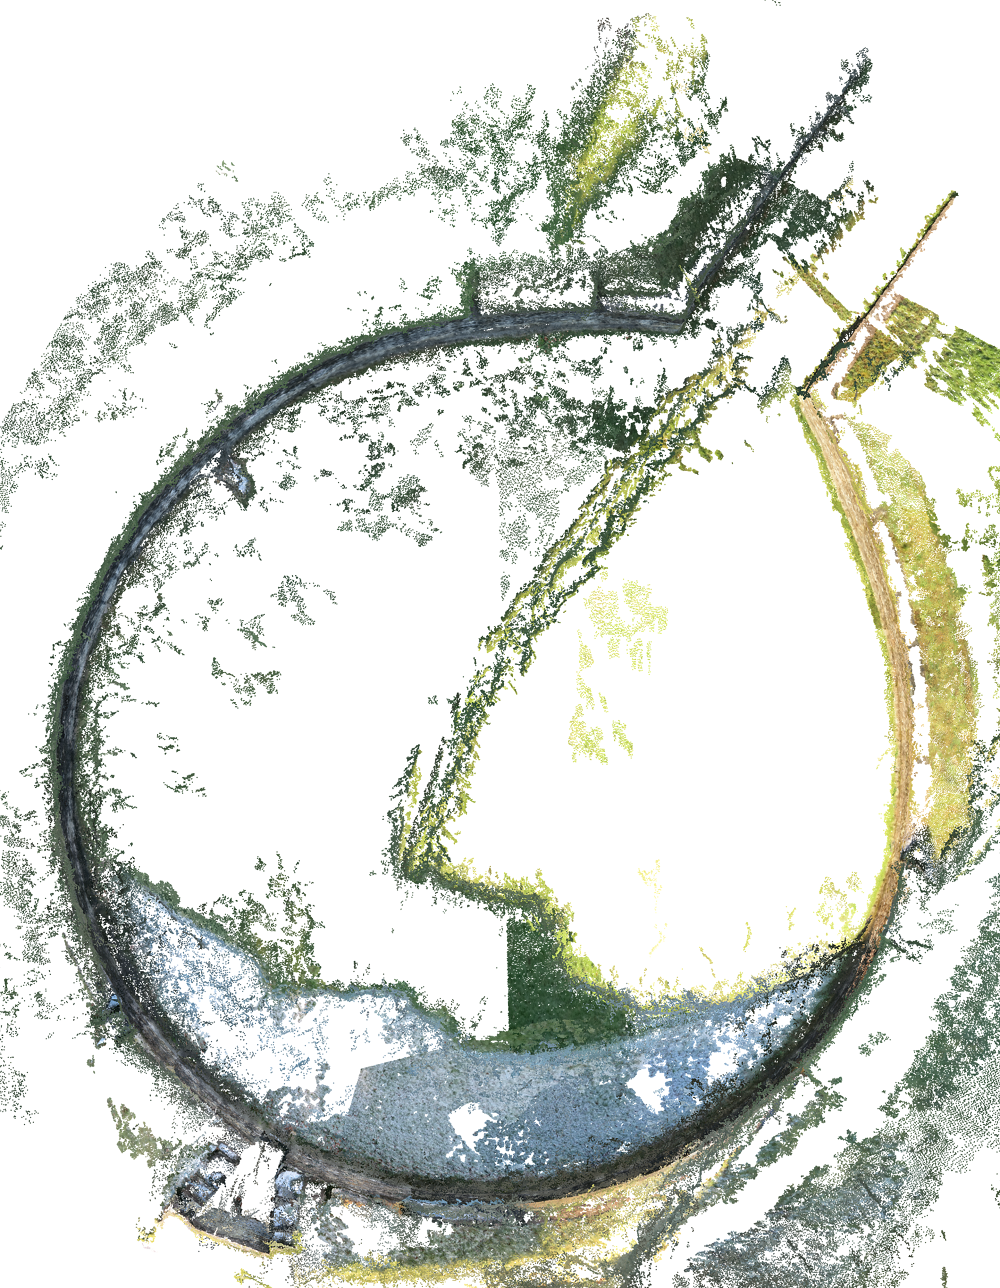
\includegraphics[width=\textwidth]{amphi_ortho_meshl_sm}
						\caption{Orthofoto der Point Cloud}
					\end{subfigure}	
					\begin{subfigure}{0.4\textwidth}
						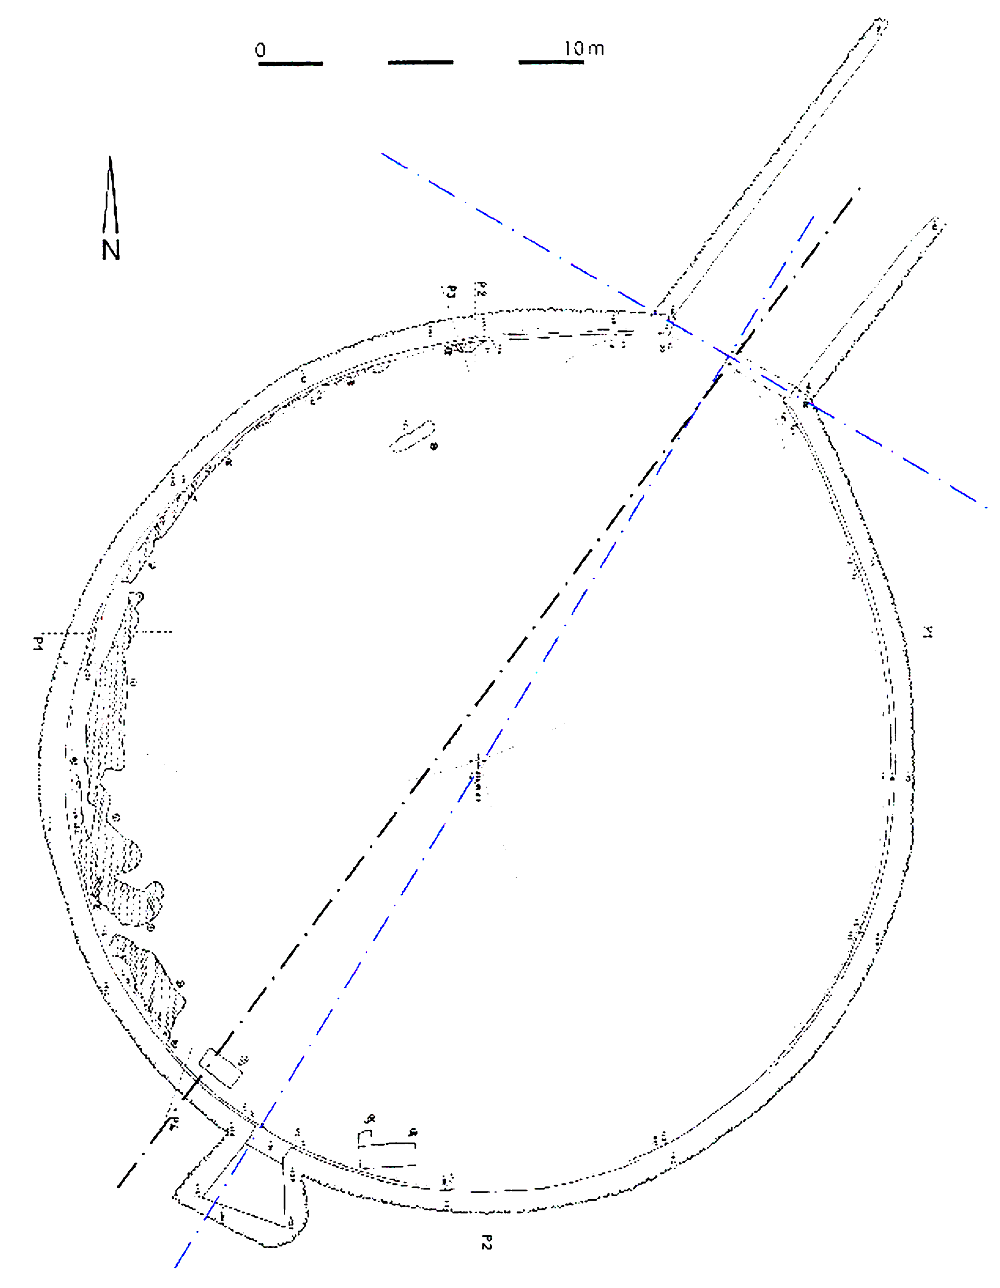
\includegraphics[width=\textwidth]{amphi_ortho_plan_edit_sm}
						\caption{Plan des Theaters}
					\end{subfigure}
					\begin{subfigure}{\textwidth}
						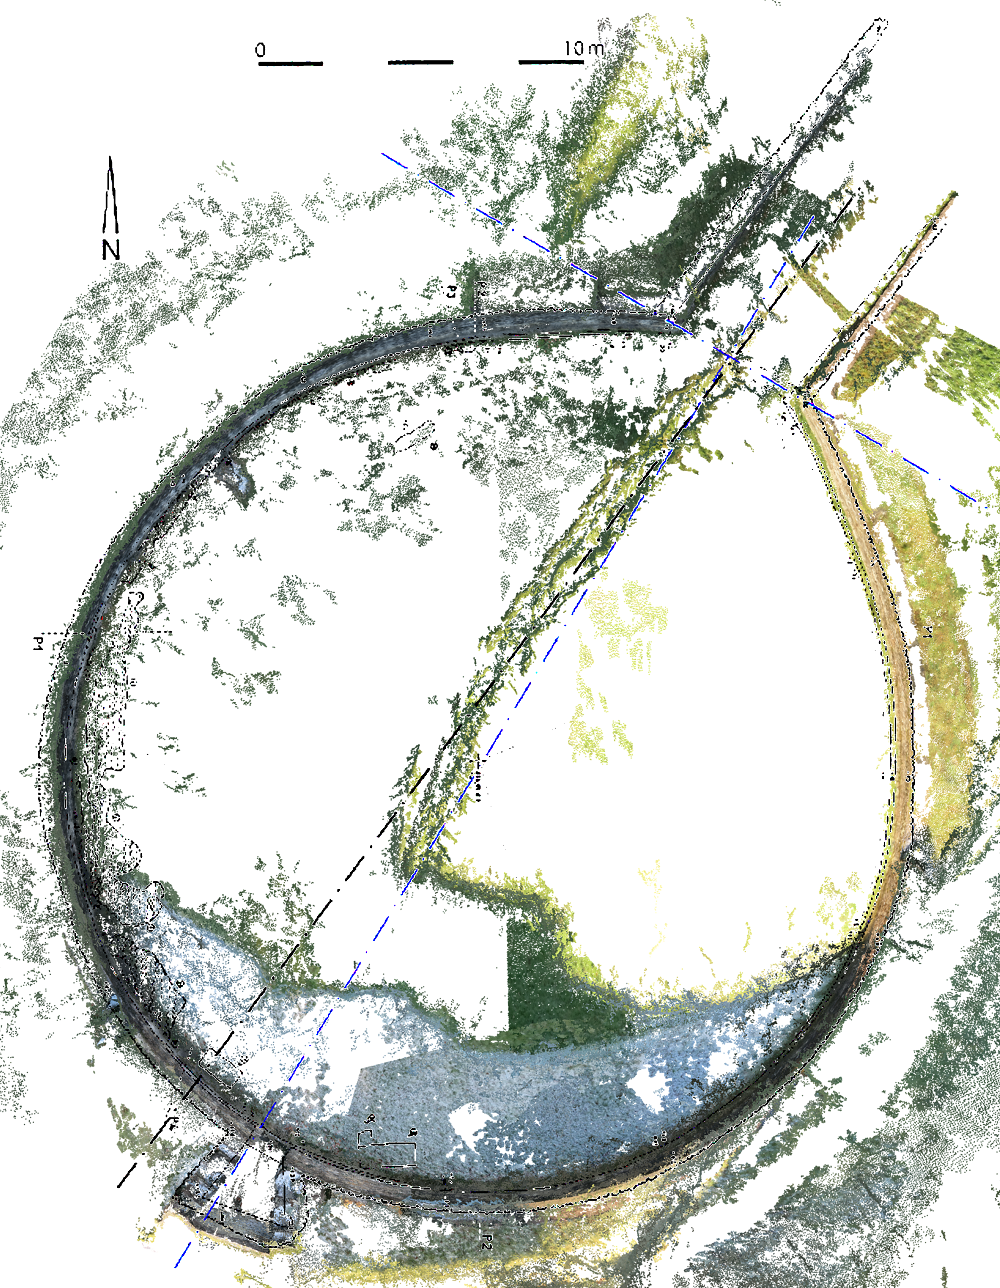
\includegraphics[width=\textwidth]{amphi_ortho_mesh_sm}
					\end{subfigure}
					\caption[Überlagerung von Plan und Orthofoto. Plan aus \cite{engehalb}]{Überlagerung von Plan und Orthofoto. Die Abweichung ist unten links ersichtlich.}
					\label{ortho_amphi_meshlab}
				\end{figure}
		\subsection{Test mit vorhandenen Bildern} \label{res:test_vorhandene_bilder}
			TODO: Welche Bilder?
			
	\section{Scans kleiner Objekte}
		SfM erscheint auch attraktiv um einzelne kleine Objekte, wie Knochen oder Keramikfragmente, 3D zu erfassen und dokumentieren. In sieben Versuchen mit verschiedenen Objekten ist es allerdings weder mit \dronarch\ noch mit PhotoScan\autorefu{app:photoscan} gelungen eine vollständige Rekonstruktion zu machen. Deshalb kann das Verfahren auf kleine Objekte angewendet so nicht als brauchbare Alternative zu Laserscannern betrachtet werden
		
	\chapter{Fazit}
	Die Ergebnisse aus \autoref{resultate} und die vorangehende Forschung, die in \autoref{related:work} diskutiert wird, legen nahe, dass SfM und MvS Verfahren in der Archäologie ausgesprochen nützlich sind.
	
	\section{Auswertung}	
		Ergebnissen aus \autoref{res:fall} können nun mit der Fragestellung in \autoref{frag:ziel} ausgewertet werden.
		
		\paragraph{Mehrwert}
			Das Modell ist trotz schlechten Aufnahmebedingungen gut genug um Details in der Mauer und die geometrische Form des Theaters gut zu erkennen.
			Durch die Löcher im Boden ist es für Öffentlichkeitsarbeit vermutlich nicht gut genug, gibt aber schon so dem ungeübten Auge eine gute Vorstellung der Situation.
			Erstrebenswert wäre eine gleichmässigere Verteilung der Punkte um damit ein Mesh bilden zu können.
			
			Der Detailgrad reicht an den meisten Stellen um einzelne Steine der Mauer zu erkennen und damit um beispielsweise deren Grösse oder Farbe zu bestimmen.
						
		\paragraph{Aufwand}
			Das Aufnehmen der Fotos war in weniger als 20 Minuten getan und kann mit etwas Übung noch schneller vonstatten gehen, da für eine vergleichbare Qualität der Rekonstruktion auch die Hälfte der Bilder genügt hätten.
			Weniger Bilder verkürzen auch die Berechnungszeit von bis zu 20 Stunden drastisch, da die benötigte Zeit nicht linear, sondern stärker, zunimmt.
			Die lange Rechenzeit ist wenig problematisch, da die unbeaufsichtigt gemacht werden kann, sie führt aber zu einem Stromverbrauch von knapp 10KWh pro Rekonstruktion.
						
		\paragraph{Qualität}
			Die Überlagerung eines Orthofotos und Planes in \autoref{ortho_amphi_meshlab} war die einzige angewandte Fehlermessung im Rahmen dieser Arbeit und die Aussagekraft dieses Vergleichs ist beschränkt. Das Modell scheint demnach keine grossen Abweichung zu haben, die Geometrie stimmt gut überein.
			Einzelne abweichende Punkte können bei der Rekonstruktion durch anpassen von Parametern mehr oder weniger streng verworfen werden, was aber auch korrekte Punkte entfernen kann. Hier braucht es etwas Erfahrung um ein bestmögliches Resultat zu erhalten.
			
		\paragraph{Integration}
			Mit Hilfe eines Planes wurde ein Modell skaliert und orientiert\autorefu{ortho_amphi_meshlab}. Diese fand aber wegen dem Plan als 2D Referenz nur in zwei Dimensionen statt. Eine korrekte Referenzierung müsste über vermessene Kontrollpunkte passieren.
			Die verwendete Software Meshlab\citeu{meshlab:home} unterstützt diese Ansätze ohne zusätzliche Erweiterungen zu wenig, weitere Nachforschungen in diesem Punkt wären notwendig.
			
		\paragraph{Schwierigkeiten}
			Die Hauptschwierigkeit ist das Erstellen der Fotos, da nie klar ist, ob die Rekonstruktion mit den gemachten Bildern funktionieren wird, oder ob noch mehr Bilder benötigt werden. Auch hier wird Erfahrung helfen effizienter und sicherer arbeiten zu können.
			
			Diese Unsicherheit ist ein wesentlicher Kritikpunkt an dem Verfahren, denn durch die langen Rechenzeit kann nicht vor Ort überprüft werden ob die Rekonstruktion gelingt. Dies ist eine starke Einschränkung für die Verwendung zu einer lückenlosen Dokumentation.
				
	\section{Weitere Forschung}
		Das Potential von 3D Scans, insbesondere von SfM, ist damit natürlich längst nicht ausgeschöpft. Dieser Ansatz zu einer effizienten exakten Dokumentationsweise und intuitiven natürlichen Darstellung bietet noch viele Möglichkeiten zur Verbesserung.
		
		\paragraph{Verbesserte Visualisierung}
			Snavley \etal\ verwenden neben Point Clouds in ihrer Darstellung von Monumenten auch die originalen Fotos\citeu{Snavely:2006:PTE:1179352.1141964}. Dem Nutzer wird direkt in dem 3D Modell das Foto und dessen Position angezeigt. Damit werden Fotos direkt in das 3D Modell integriert und die Interpretation stark vereinfacht.
			
		\paragraph{3D Druck}
			Die Kantonsarchäologie Aargau hat von Vindonissa ein 3D Modell erstellt und dieses von einem 3D Drucker im Massstab 1:450 nachbauen lassen\citeu{arch:print_vindonissa}. Das selbe Verfahren lässt sich auf beliebige 3D Modelle anwenden, so auch auf Meshes, die mit SfM erstellt wurden.
			
		\paragraph{Automatisierte Bilderfassung}
			\dronarch\ wurde mit der Idee von automatischer Bilderfassung mittels Drohnen geboren und dieser Ansatz bietet viele Möglichkeiten. Mit Drohnen könnten die Fotos automatisch und periodisch erstellt werden und schwierig zugängliche Stellen problemlos erfasst werden. Das ein autonomes Navigieren auch mit günstigen Drohnen möglich ist wurde bereits gezeigt\citeu{klein07parallel, engel14ras, alvarez14iser}, die verfügbare Implementierung davon hat sich aber noch als zu wenig robust herausgestellt.
			
			Neben Drohnen könnten stationäre Kameras, die periodisch Fotos machen, eingesetzt werden.

		\paragraph{Performance Verbessern}
			Die in \dronarch\ verwendete Software ist bei weitem nicht die schnellstmögliche und die Rechenzeit könnte durch Optimierungen verkürzt werden. Im Moment laufen viele Schritte nicht parallel und so könnte man etwa mit \emph{Multicore Bundle Adjustment} Wu \etal\citeu{Wu11multicorebundle} den SfM Teil parallelisieren.
	
	
	\begin{appendix}
		\chapter{Begriffe}
		\section{Point Cloud}\label{app:point_cloud}
		Eine Point Cloud (Punktwolke) ist eine Menge von Punkten im 3D Raum. Die Punkte sind nicht miteinander verbunden, noch enthalten sie Informationen über Orientierung oder benachbarte Punkte. Die meisten 3D Scanner produzieren Point Clouds, die zu einem Mesh weiterverarbeitet werden können.
		Sind die Punkte dicht beieinander, spricht man von einer \emph{dense} (dicht) Point Cloud. Ansonsten nennt man sie \emph{sparse} (licht, locker).
		
		\section{Mesh}\label{app:mesh}
		Verbindet man mehrere Punkte zu einer Fläche, meist zu Dreiecken, enthält man ein Mesh. Dies hat eine klare Orientierung und setzt Punkte in Verbindung mit ihren Nachbarn. Enthält ein Mesh keine Löcher, nennt man es watertight (wasserdicht).		
	\end{appendix}
	
	%	\addcontentsline{toc}{section}{\numberline{}List of Figures}
	%	\listoffigures
	
	\addcontentsline{toc}{section}{\numberline{}Bibliography}
%		\bibliographystyle{apalike}
%	\bibliographystyle{IEEEtran}
	\bibliographystyle{nick_2}
	\nocite{*}
%	\printbibliography
	\bibliography{dronarch}
	

	
\end{document}